\documentclass[a4paper,12pt]{article}
\usepackage{graphicx} 
\usepackage{geometry}
\usepackage{titlesec} 
\setlength{\parskip}{1em} 
\titleformat{\section}{\normalfont\LARGE\bfseries}{\thesection}{1em}{}
\usepackage{titlesec}
\usepackage{titletoc}
\usepackage{hyperref} 
\usepackage{booktabs}
\usepackage{array} 
\usepackage{lmodern}
\usepackage{caption}
\usepackage{amsmath}
\geometry{
    top=0.5in,
    bottom=1in, % Adjust the bottom margin,
    headheight=0pt, % Adjust the header height if needed
    footskip=20pt, % Adjust footskip to reduce space after page number
}
\usepackage{float}


\begin{document}
\thispagestyle{empty} 
% University logo at the top
\begin{center}
    
\includegraphics[width=0.12\textwidth]{photos/logo.png}  \\[1.5em]
    {\LARGE Noakhali Science \& Technology University} \\
    Department of Computer Science \& Telecommunication Engineering
\end{center}

\vspace{3.5cm}

% Title of the project report
\begin{center}
    \textbf{\huge Lab Report On:} \\[0.5em]
   \textbf{\LARGE Class modeling, Project planning, and
Risk analysis} \\[1em]
      \textbf{\Large Course Code: CSTE 3210}  \\[1.5em]
    {\large Submitted by:} \\[0.6em]
     {\large   \textbf {Group No.} : 23}  \\ [0.6em ]
     \textbf {\large Mohammad Borhan Uddin }  \\
  {\large ID: ASH2101008M}  \\ [0.6em ]
    \textbf{\large Mohammad Billal Hossain}  \\
    {\large ID: MUH2101028M}  \\ [2em]

    
    {\large Submitted to:} \\[0.6em]
    \textbf{\large Dr. Nazia Majadi} \\ 
    {\large Associate Professor} \\ 
     {Department of Computer Science \& Telecommunication Engineering} \\ 
\end{center}

\vspace{5cm}

\begin{center}
    \textbf{\LARGE Date : May 18, 2025}
\end{center}
\thispagestyle{empty} 

\tableofcontents

\thispagestyle{empty}
\newpage

\setcounter{page}{1} 

\section{Requirement analysis}
This section focuses on analyzing the system requirements using various modeling techniques to understand and document how the system will function and interact with users and data.

\subsection{Flow Models}
Flow models use Data Flow Diagrams (DFDs) to represent the flow of data within the system, illustrating processes, data stores, external entities, and data flows.

\noindent \textbf{(i) Level 0 DFD} \\
A Level 0 DFD, also known as a context diagram, provides a high-level overview of the entire system as a single process interacting with external entities (e.g., users, admins, employees). 
\begin{figure}[H]
    \centering
    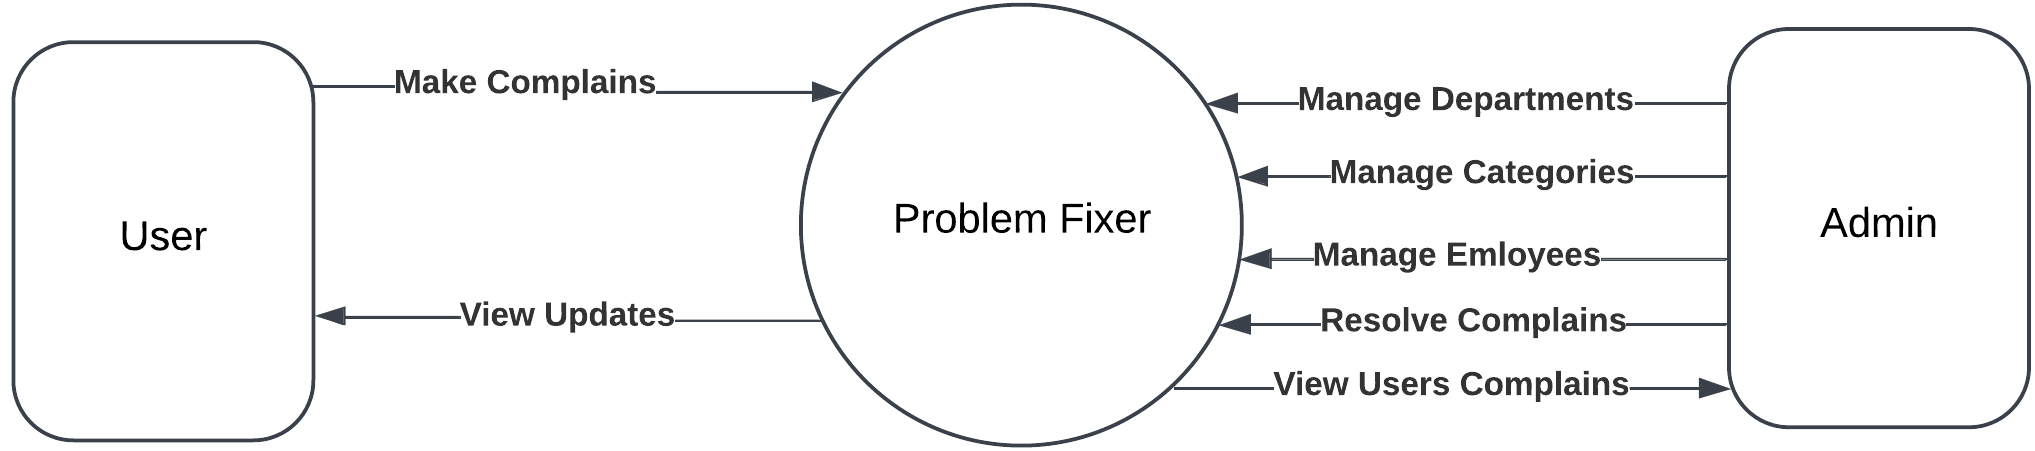
\includegraphics[width=1\linewidth]{photos/dfd-0.png}
    \caption{Level 0 DFD}
    \label{fig:enter-label}
\end{figure}

\noindent \textbf{(ii) Level 1 DFD} \\
A Level 1 DFD decomposes the single process from the Level 0 DFD into major subprocesses, showing how data flows between them. 
\begin{figure}[H]
    \centering
    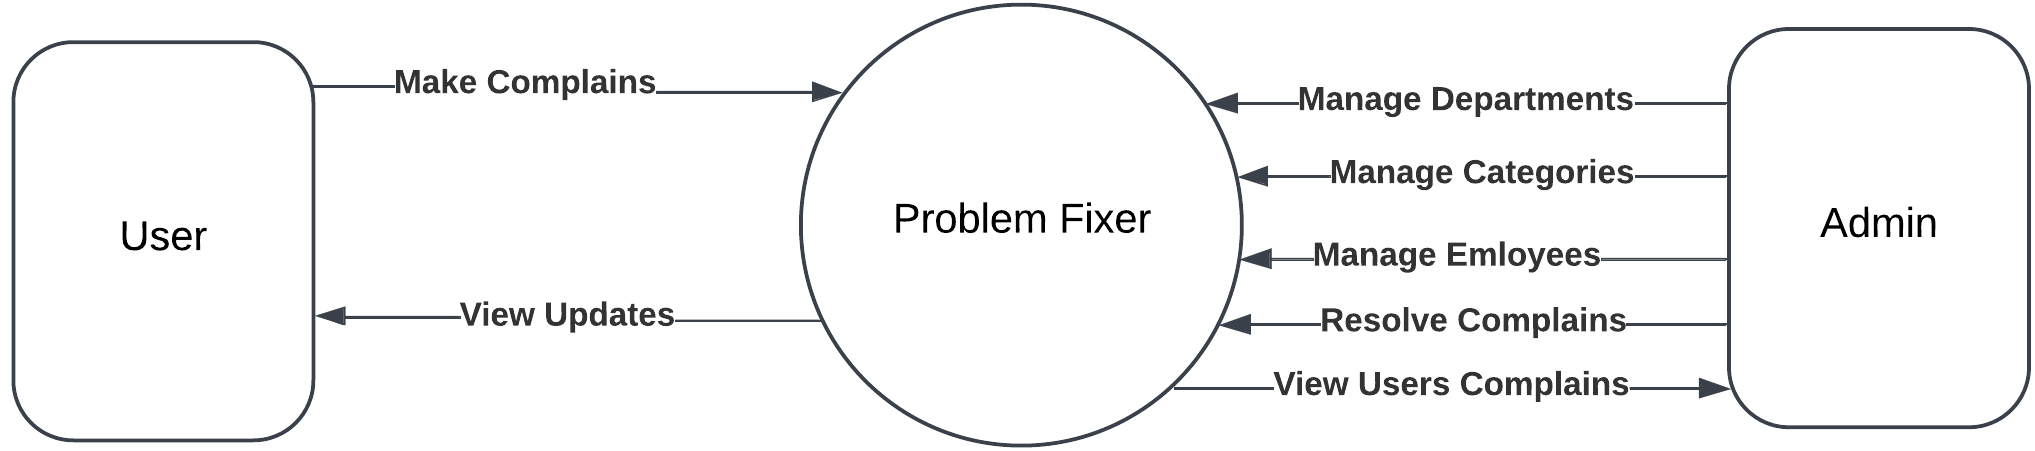
\includegraphics[width=1\linewidth]{photos/dfd-0.png}
    \caption{Level 1 DFD}
    \label{fig:enter-label}
\end{figure}

\noindent \textbf{(iii) Level 2 DFD} \\
A Level 2 DFD further decomposes one or more processes from the Level 1 DFD into finer subprocesses.
\begin{figure}[H]
    \centering
    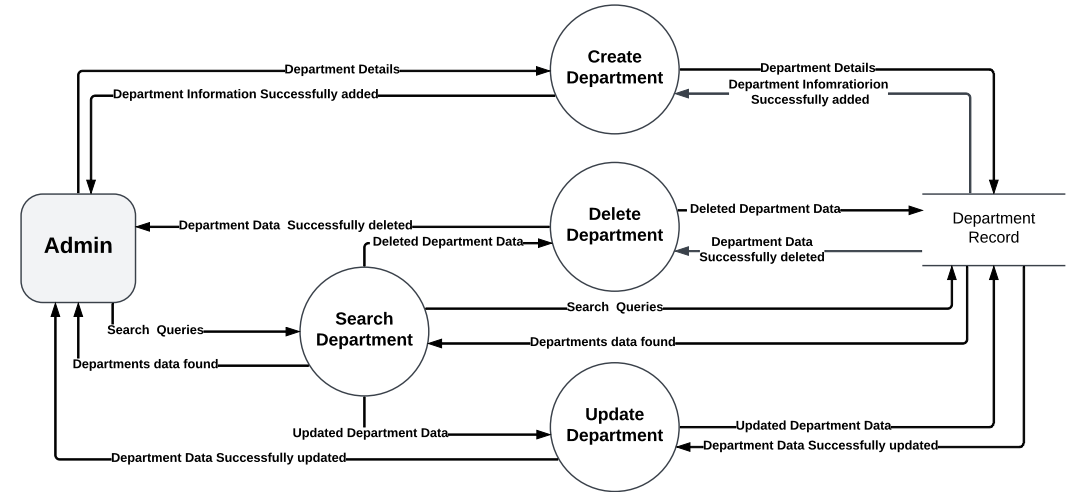
\includegraphics[width=1\linewidth]{photos/dfd-2-department.png}
    \caption{Level 2 Data Flow Diagram: Administrative Management of Departments}
    \label{fig:enter-label}
\end{figure}
\begin{figure}[H]
    \centering
    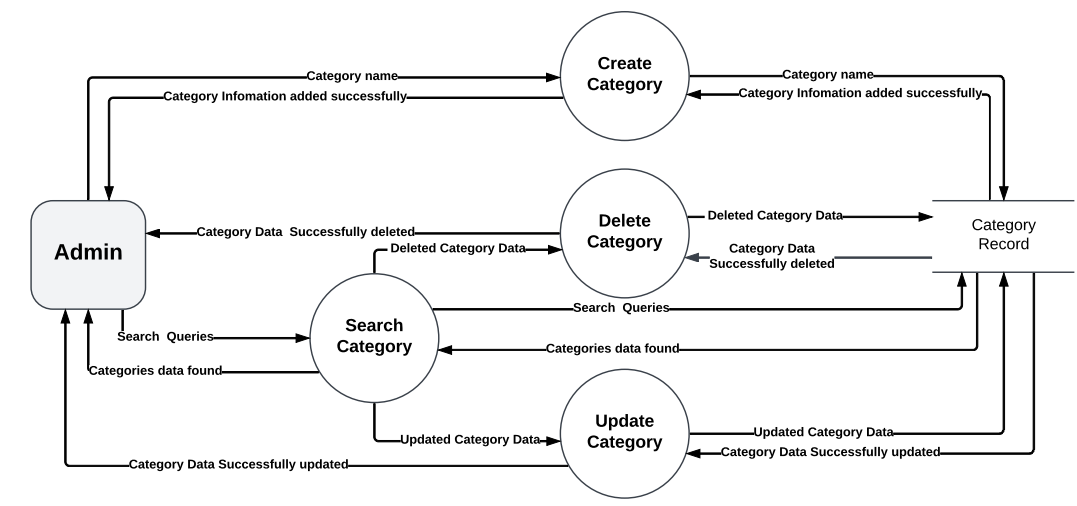
\includegraphics[width=1\linewidth]{photos/dfd-2-category.png}
    \caption{Level 2 Data Flow Diagram: Administrative Management of Categories}
    \label{fig:enter-label}
\end{figure}
\begin{figure}[H]
    \centering
    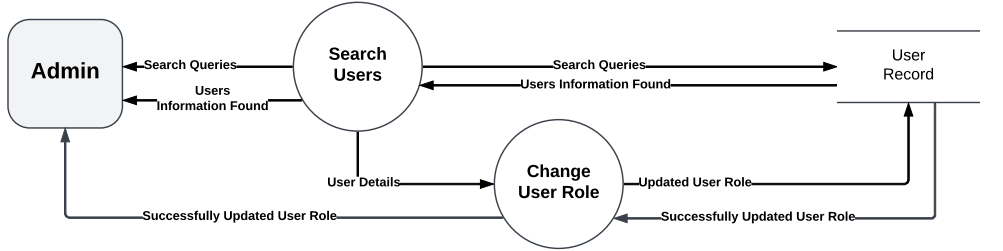
\includegraphics[width=1\linewidth]{photos/dfd-2-user.png}
    \caption{Level 2 Data Flow Diagram: Administrative Management of User}
    \label{fig:enter-label}
\end{figure}
\begin{figure}[H]
    \centering
    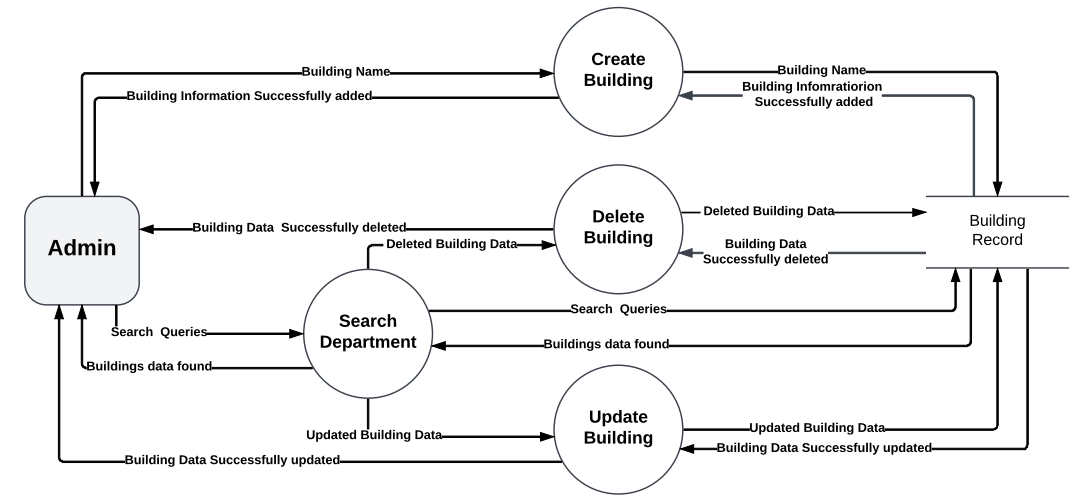
\includegraphics[width=1\linewidth]{photos/dfd-2-building.png}
    \caption{Level 2 Data Flow Diagram: Administrative Management of Buildings}
    \label{fig:enter-label}
\end{figure}

\begin{figure}[H]
    \centering
    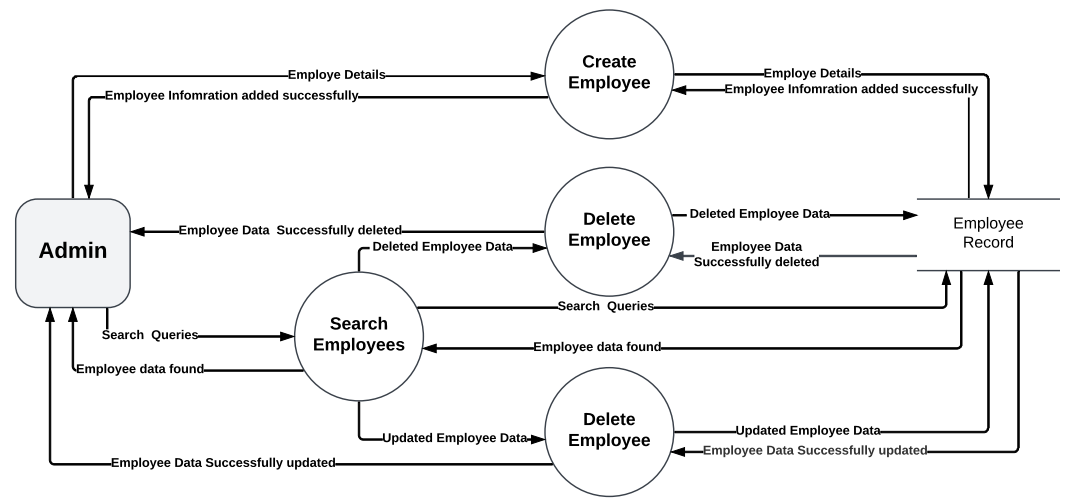
\includegraphics[width=1\linewidth]{photos/dfd-2-employee.png}
    \caption{Level 2 Data Flow Diagram: Administrative Management of Employee}
    \label{fig:enter-label}
\end{figure}
\begin{figure}[H]
    \centering
    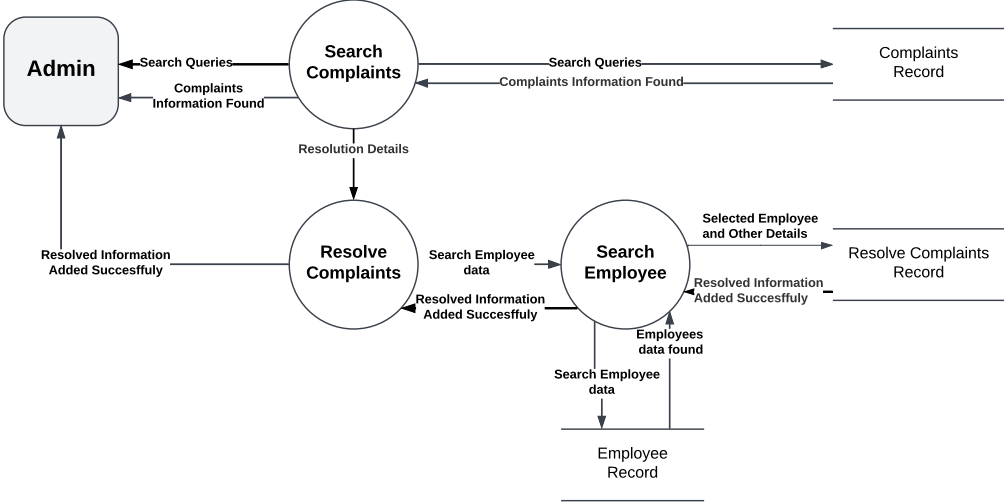
\includegraphics[width=1\linewidth]{photos/dfd-2-resolve.png}
    \caption{Level 2 Data Flow Diagram: Administrative Management of Complaint Resolution }
    \label{fig:enter-label}
\end{figure}

\begin{figure}[H]
    \centering
    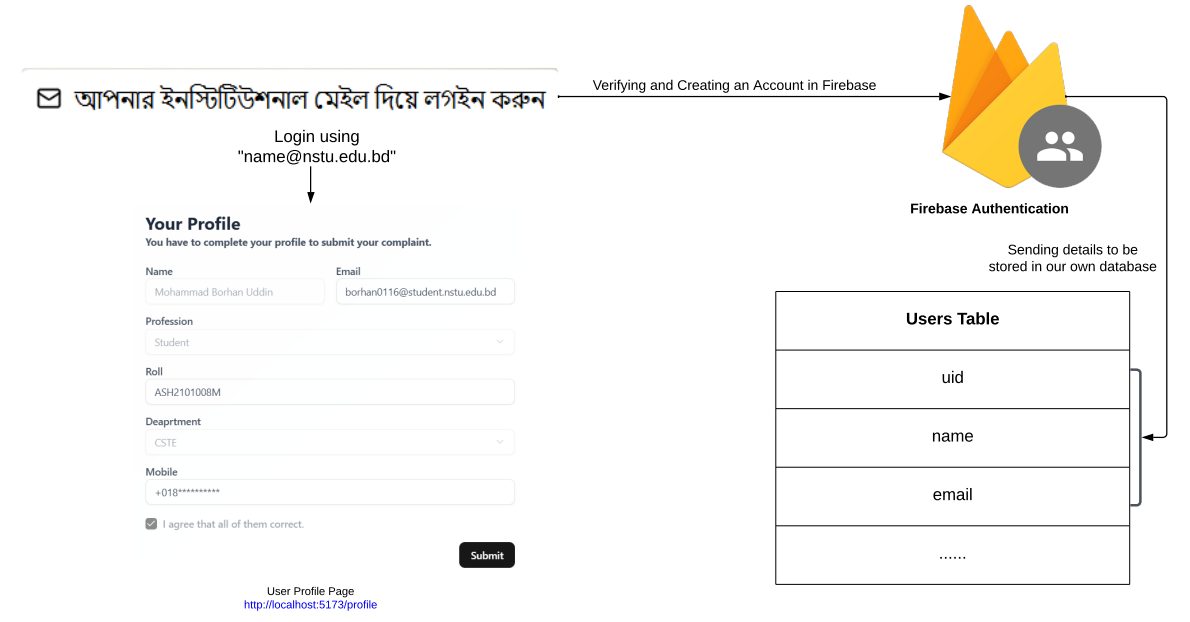
\includegraphics[width=1\linewidth]{photos/dfd-2-auth.png}
    \caption{Level 2 Data Flow Diagram: Authentication System }
    \label{fig:enter-label}
\end{figure}

\begin{figure}[H]
    \centering
    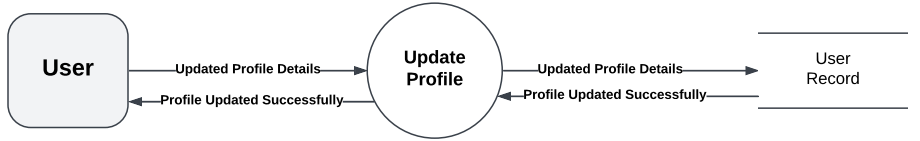
\includegraphics[width=1\linewidth]{photos/dfd-2-update-profile.png}
    \caption{Level 2 Data Flow Diagram: User Profile Management }
    \label{fig:enter-label}
\end{figure}

\begin{figure}[H]
    \centering
    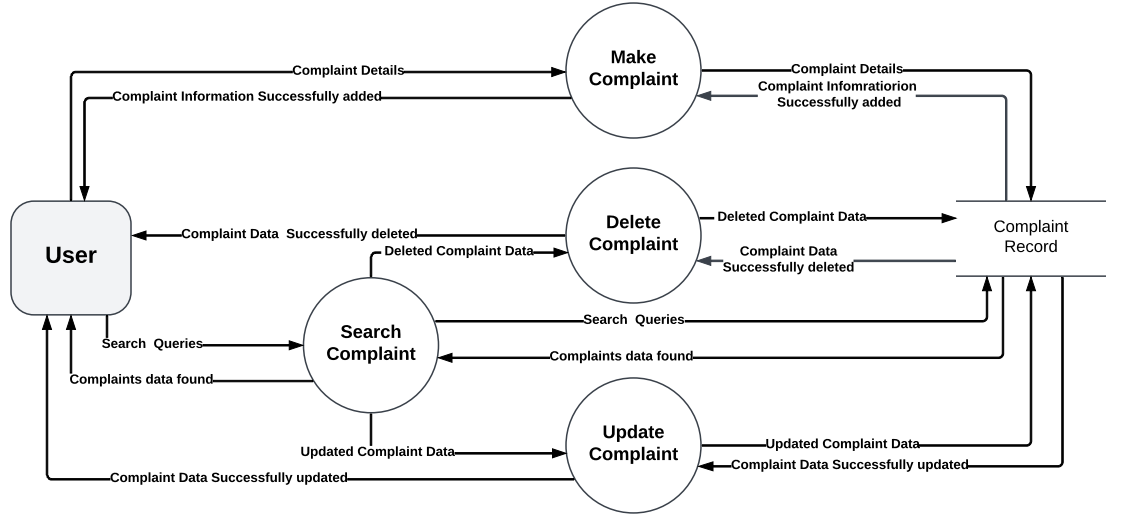
\includegraphics[width=1\linewidth]{photos/dfd-2-complaint.png}
    \caption{Level 2 Data Flow Diagram: User Management of Complaints }
    \label{fig:enter-label}
\end{figure}

\subsection{Class-Based Models}
Class-based models focus on the structural aspects of the system, defining entities, their attributes, relationships, and responsibilities.
\\ \\ 
\noindent \textbf{(i) Entity-Relationship Diagram} \\
An Entity-Relationship (ER) Diagram represents the database structure of the system, showing entities , their attribute, and relationships.
\begin{figure}[H]
    \centering
    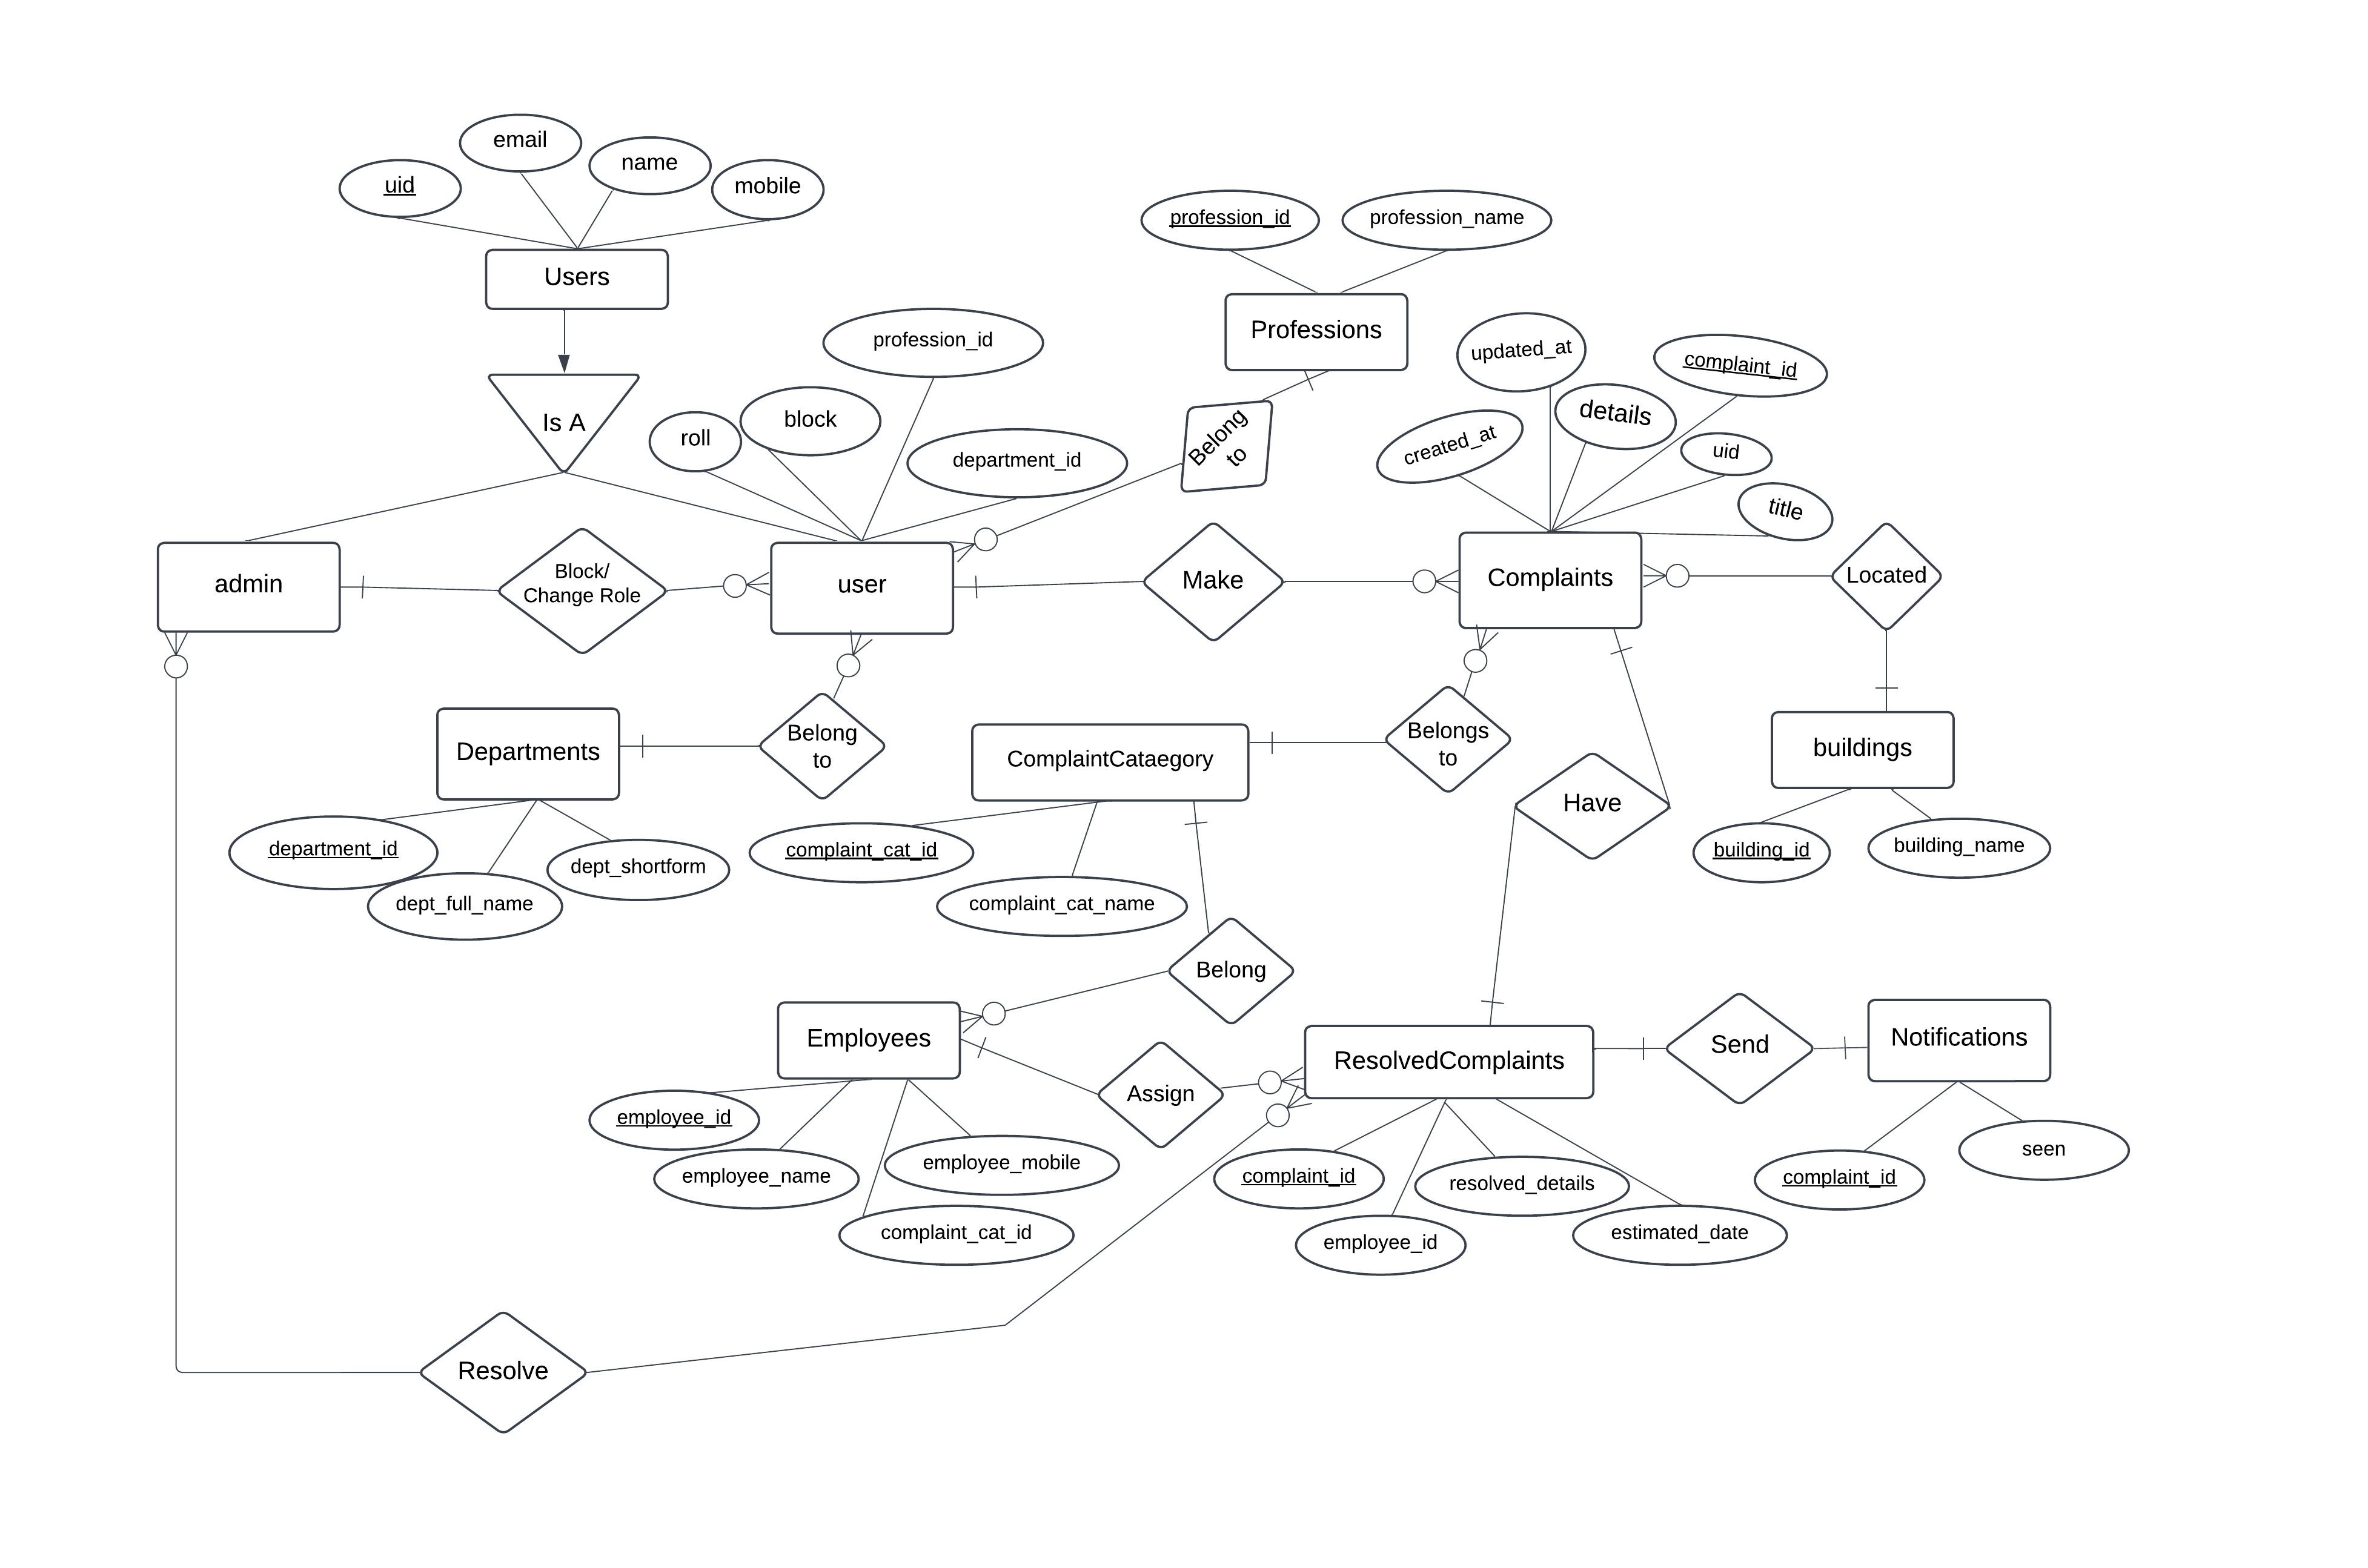
\includegraphics[width=1\linewidth]{photos/erd.png}
    \caption{ER Diagram}
    \label{fig:enter-label}
\end{figure}

\begin{figure}[H]
    \centering
    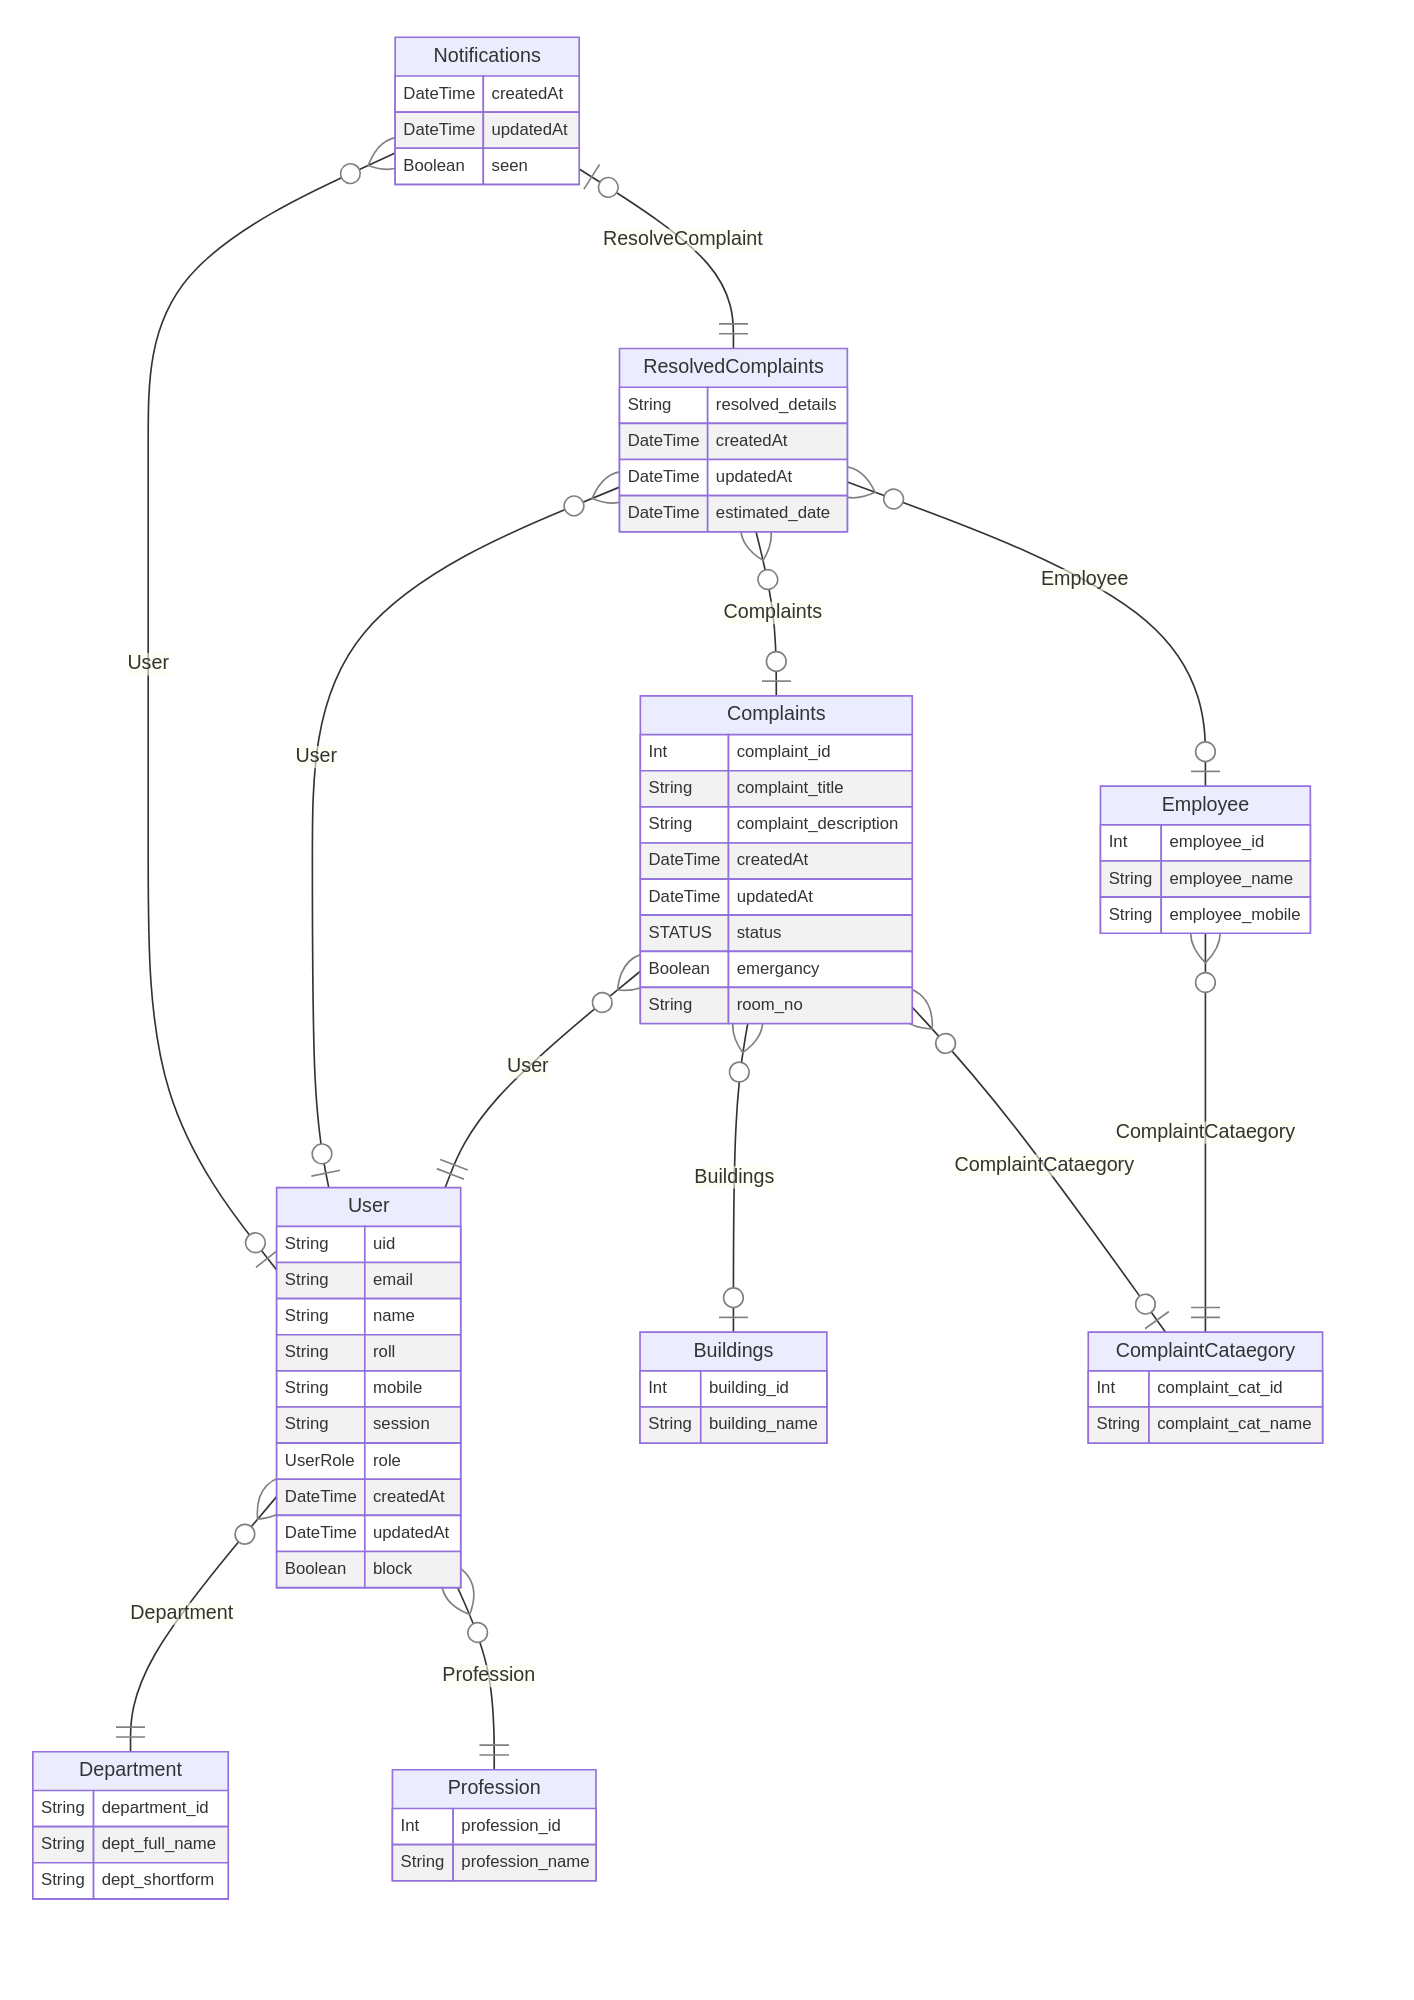
\includegraphics[width=1\linewidth]{photos/er-schema.png}
    \caption{Entity-Relationship Schema Diagram}
    \label{fig:enter-label}
\end{figure}



 \noindent \textbf{(i) Class Diagram} \\
A UML Class Diagram models the system’s classes, their attributes, methods, and relationship.
\begin{figure}[H]
    \centering
    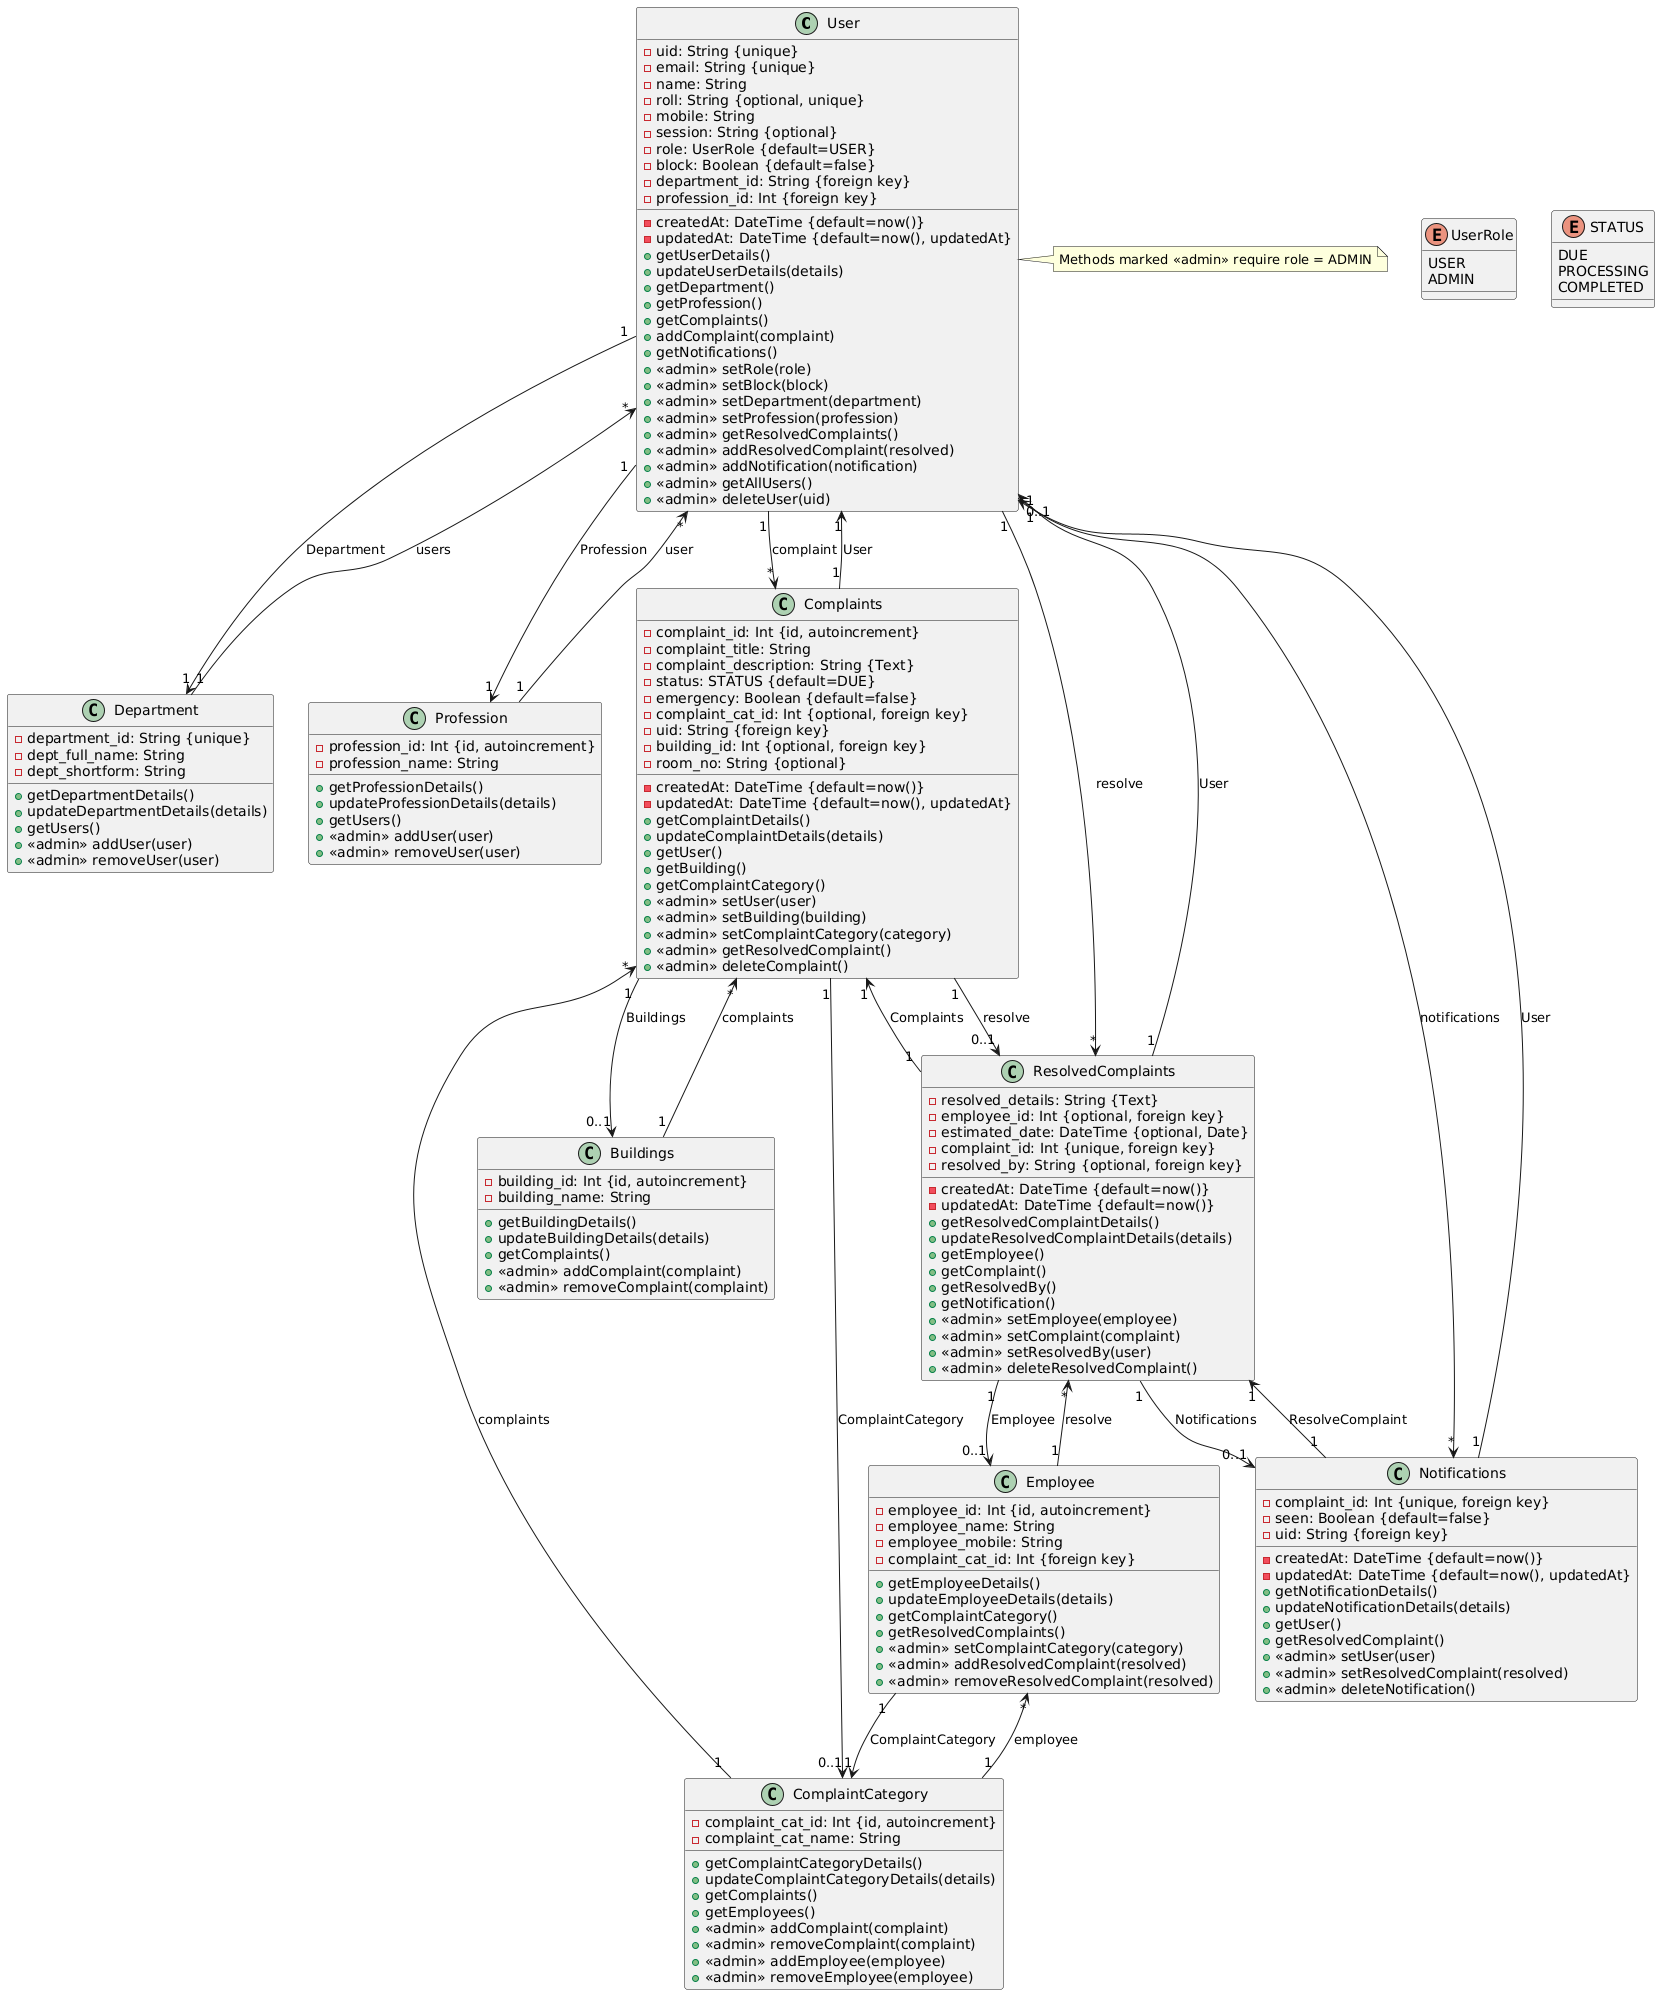
\includegraphics[width=1\linewidth]{photos/class-diagram}
    \caption{Class Diagram}
    \label{fig:enter-label}
\end{figure}

 \noindent \textbf{(iii) Class-Responsibility Collaboration (CRC) Modeling} \\
CRC (Class-Responsibility-Collaboration) modeling identifies classes, their responsibilities (what they d), and collaborators (other classes they interact with).
\begin{figure}[H]
    \centering
    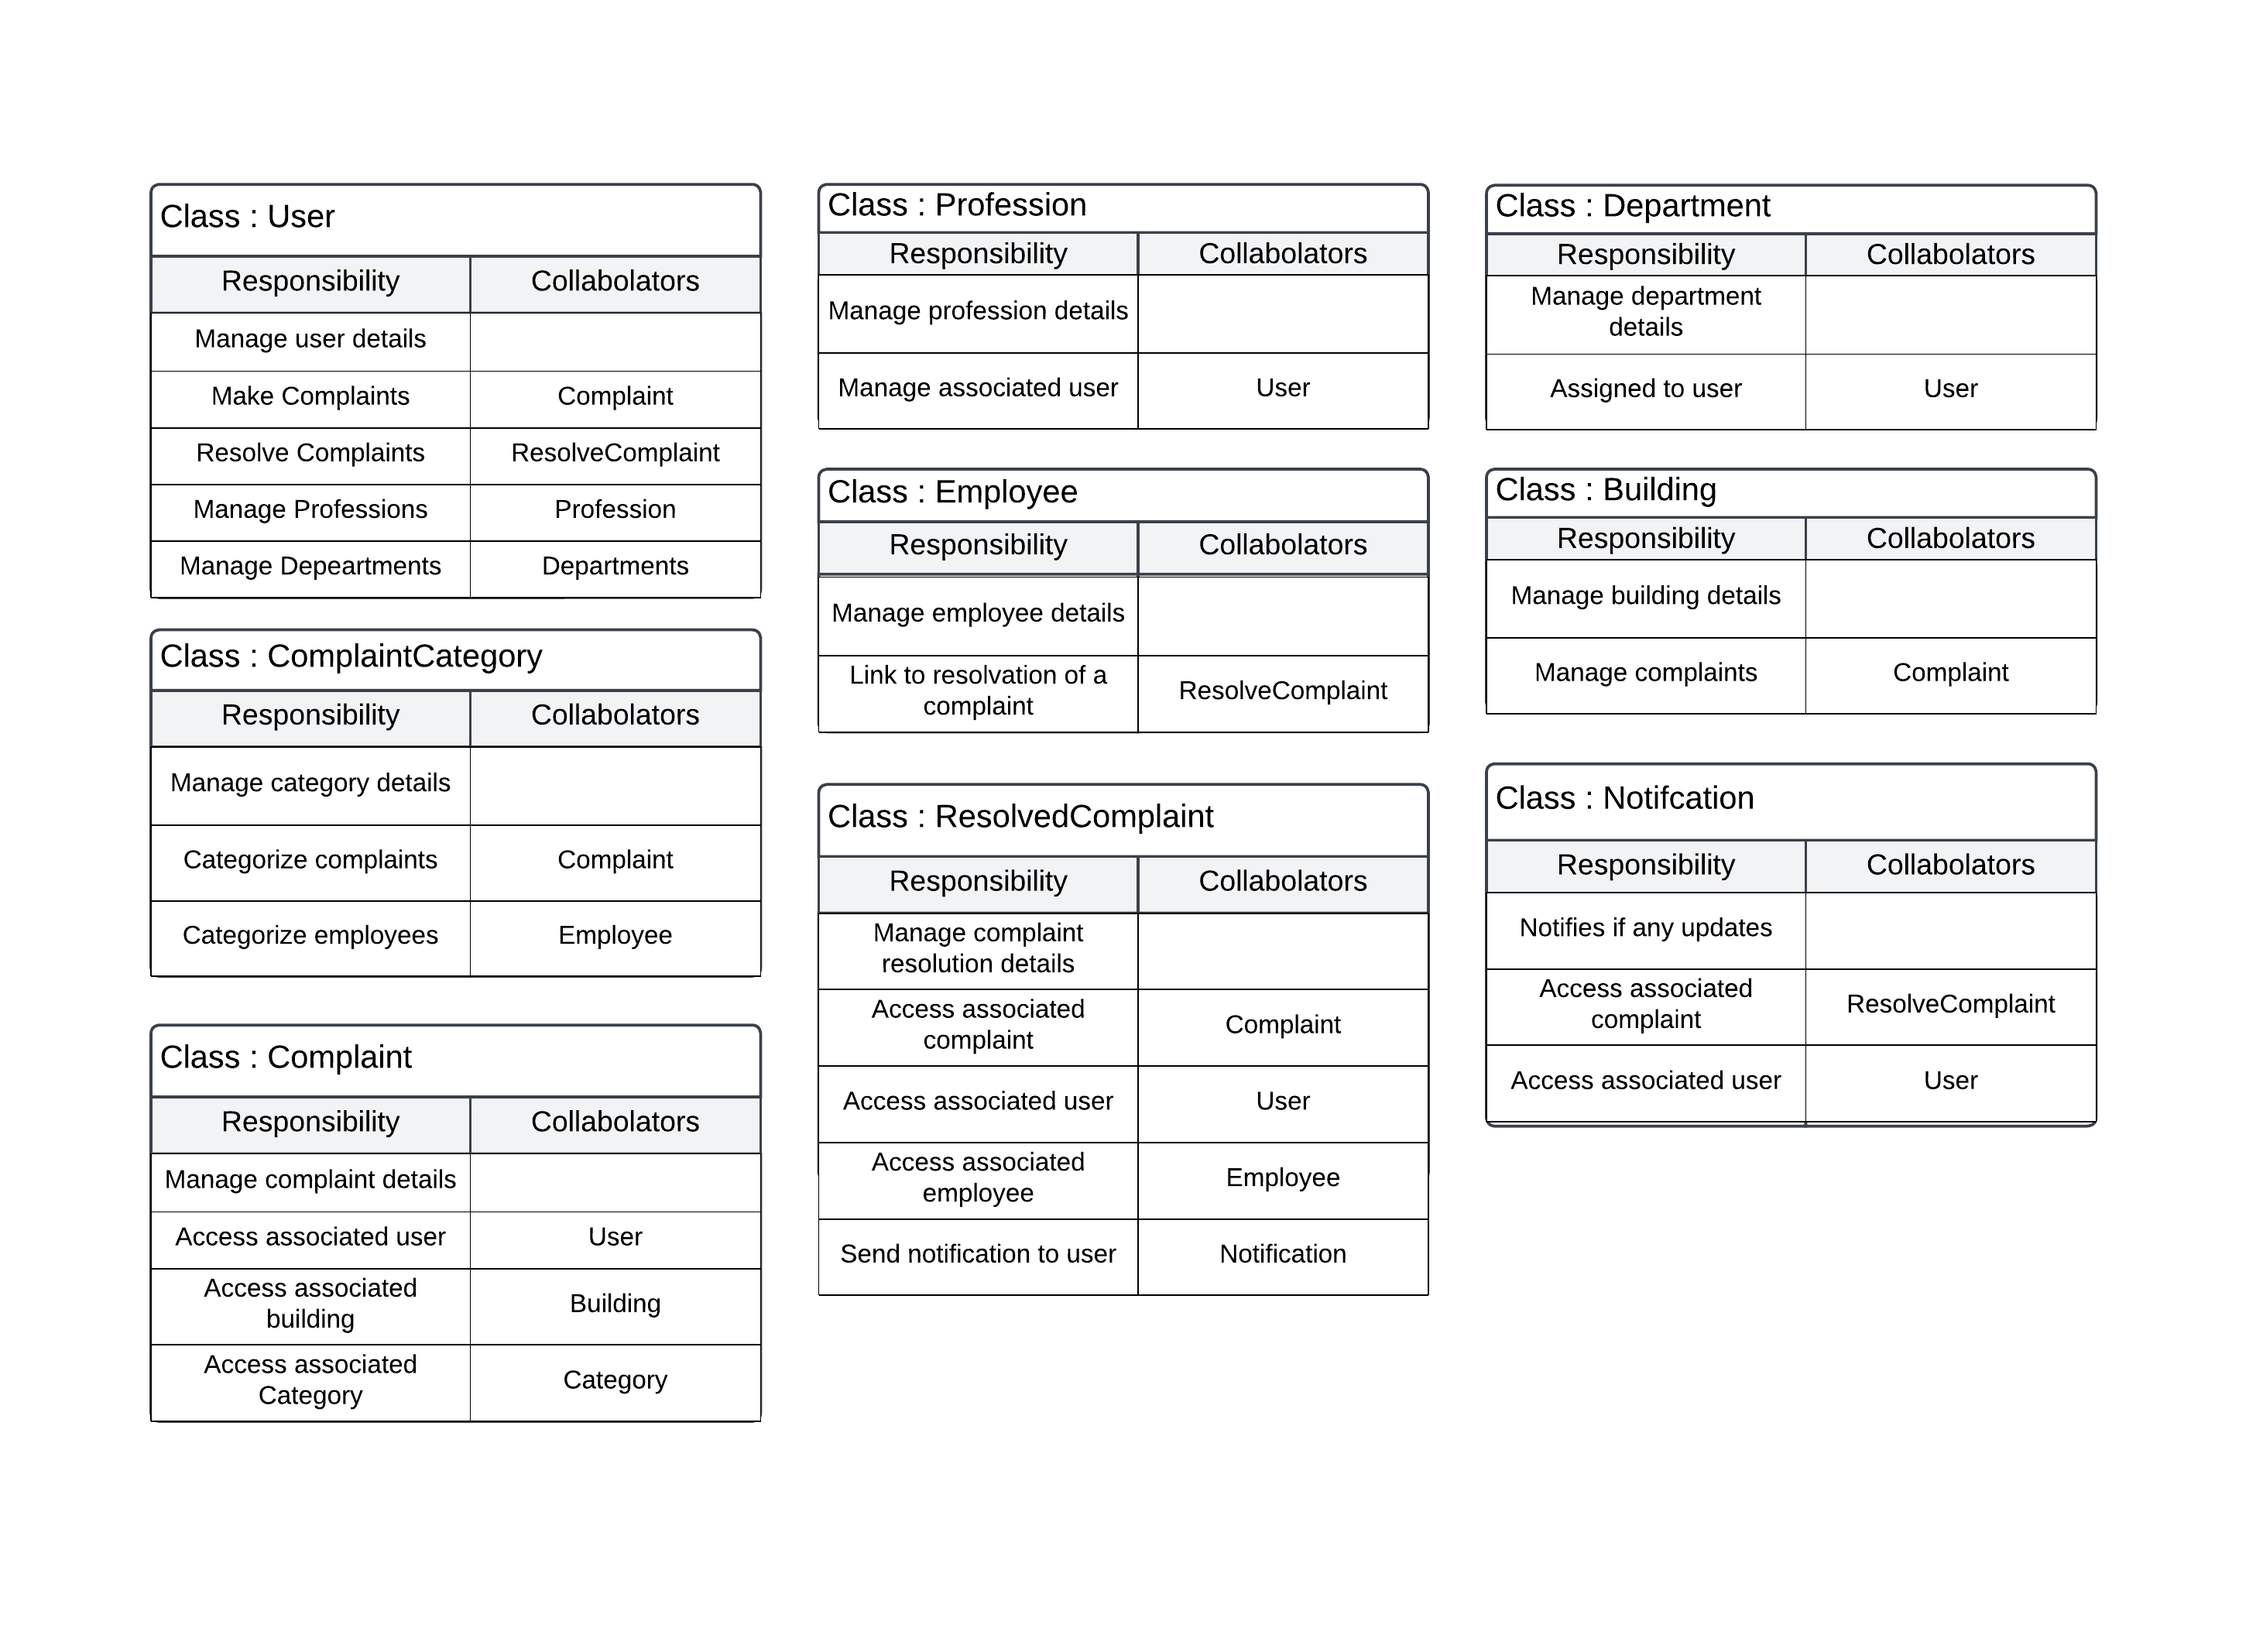
\includegraphics[width=1\linewidth]{photos/crc.png}
    \caption{Class Diagram}
    \label{fig:enter-label}
\end{figure}

\section{Project Planning}
This section outlines the planning process for developing the system, ensuring it is completed on time, within budget, and with adequate resources.

\subsection{WBS (Work Breakdown Structure)}
The WBS breaks the project into smaller, manageable tasks organized hierarchically. For the Complaint Management System, this includes phases like Initiation, Design, Development,

% Level 1: Complaint Management System Development
\paragraph*{Level 1: Complaint Management System Development}

% Level 2: Project Initiation
\paragraph*{Level 2: Project Initiation}
\begin{itemize}
    \item Define project scope and objectives
    \item Identify stakeholders (users, admins, employees)
    \item Create system requirements document
\end{itemize}

% Level 2: System Design
\paragraph*{Level 2: System Design}
\begin{itemize}
    \item Design database schema (e.g., User, Complaints tables)
    \item Develop UML class diagrams and CRC model
    \item Define user interface mockups
\end{itemize}

% Level 2: System Development
\paragraph*{Level 2: System Development}
\begin{itemize}
    \item Implement User module (authentication, profile management)
    \item Implement Complaints module (filing, status tracking)
    \item Implement Admin module (user management, resolution)
    \item Integrate Department and Profession modules
    \item Develop Notification system
\end{itemize}

% Level 2: Testing
\paragraph*{Level 2: Testing}
\begin{itemize}
    \item Unit testing (each module)
    \item Integration testing (cross-module interactions)
    \item User acceptance testing (UAT)
\end{itemize}

% Level 2: Deployment
\paragraph*{Level 2: Deployment}
\begin{itemize}
    \item Deploy to production environment
    \item Train users and admins
    \item Provide initial support
\end{itemize}

% Level 2: Maintenance
\paragraph*{Level 2: Maintenance}
\begin{itemize}
    \item Monitor system performance
    \item Handle bug fixes and updates
\end{itemize}

\subsection{Project Scheduling}
The Project Scheduling section outlines the timeline and sequencing of tasks required to
develop the Complaint Management System efficiently.
\noindent\subsubsection{CPM (Critical Path Method)} \\ 
Identifies the longest sequence of dependent tasks to determine the minimum 
project duration.

% Define new column type for centered text with fixed width
\newcolumntype{C}[1]{>{\centering\arraybackslash}m{#1}}


\begin{table}[h]
\centering
\scriptsize % Use smaller font size to ensure content fits and borders show
\begin{tabular}{|>{\raggedright\arraybackslash}m{4.0cm}|C{1.3cm}|C{2.0cm}|C{1.1cm}|C{1.0cm}|C{1.0cm}|}
\hline
\textbf{Task Name} & \textbf{Duration (Days)} & \textbf{Dependencies} & \textbf{Critical Path} & \textbf{Start Date } & \textbf{End Date} \\
\hline
Define scope/objectives & 3 & None & Yes & May 1 & May 3 \\
Identify stakeholders & 2 & Scope & Yes & May 4 & May 5 \\
Create requirements doc & 4 & Stakeholders & Yes & May 6 & May 9 \\
Design DB schema & 5 & Requirements & Yes & May 10 & May 14 \\
Develop UML/CRC & 4 & Requirements & No & May 10 & May 13 \\
Define UI mockups & 3 & Requirements & No & May 10 & May 12 \\
Implement User module & 10 & DB schema & No & May 15 & May 24 \\
Implement Complaints & 12 & DB schema & Yes & May 15 & May 26 \\
Implement Admin module & 10 & User module & No & May 25 & Jun 3 \\
Integrate Dept/Prof & 6 & User module & No & May 25 & May 30 \\
Develop Notification & 5 & User module & No & May 25 & May 29 \\
Unit testing & 8 & All & Yes & Jun 4 & Jun 11 \\
Integration testing & 6 & Unit test & Yes & Jun 12 & Jun 17 \\
User acceptance test & 5 & Integration & Yes & Jun 18 & Jun 22 \\
Deploy to production & 3 & UAT & Yes & Jun 23 & Jun 25 \\
Train users/admins & 4 & Deployment & Yes & Jun 26 & Jun 29 \\
Initial support & 5 & Training & Yes & Jun 30 & Jul 4 \\
Monitor performance & 3 & Deployment & No & Jun 26 & Jun 28 \\
Bug fixes/updates & 5 & Monitoring & No & Jun 29 & Jul 3 \\
\hline
\end{tabular}
\caption{Project Scheduling: CPM and Gantt Chart for Complaint Management System (Starting May 1,2025)}
\label{tab:project-schedule}
\end{table}
% Path 1
\textbf{Path 1} \\
 Requirements (9 days) $\rightarrow$ Database schema (5 days) $\rightarrow$ User module (10 days) $\rightarrow$ Unit testing (8 days) $\rightarrow$ Integration testing (6 days) $\rightarrow$ UAT (5 days) $\rightarrow$ Deployment (3 days) $\rightarrow$ Training (4 days) $\rightarrow$ Initial support (5 days) = 55 days

% Path 2
\textbf{Path 2} \\
 Requirements (9 days) $\rightarrow$ Database schema (5 days) $\rightarrow$ Complaints module (12 days) $\rightarrow$ Unit testing (8 days) $\rightarrow$ Integration testing (6 days) $\rightarrow$ UAT (5 days) $\rightarrow$ Deployment (3 days) $\rightarrow$ Training (4 days) $\rightarrow$ Initial support (5 days) = 57 days

% Path 3
\textbf{Path 3} \\
 Requirements (9 days) $\rightarrow$ Database schema (5 days) $\rightarrow$ Admin module (10 days) $\rightarrow$ Unit testing (8 days) $\rightarrow$ Integration testing (6 days) $\rightarrow$ UAT (5 days) $\rightarrow$ Deployment (3 days) $\rightarrow$ Training (4 days) $\rightarrow$ Initial support (5 days) = 55 days


% Critical Path
\textbf{Critical Path} \\
Path 2 (57 days) is the longest, so the project minimum duration is 57 days. Tasks on this path (e.g., Complaints module) must be completed on time to avoid delays.

\noindent\subsubsection{Gantt Chart} \\ 
A visual timeline showing task start/end dates and dependencies. 
\begin{figure}[H]
    \centering
    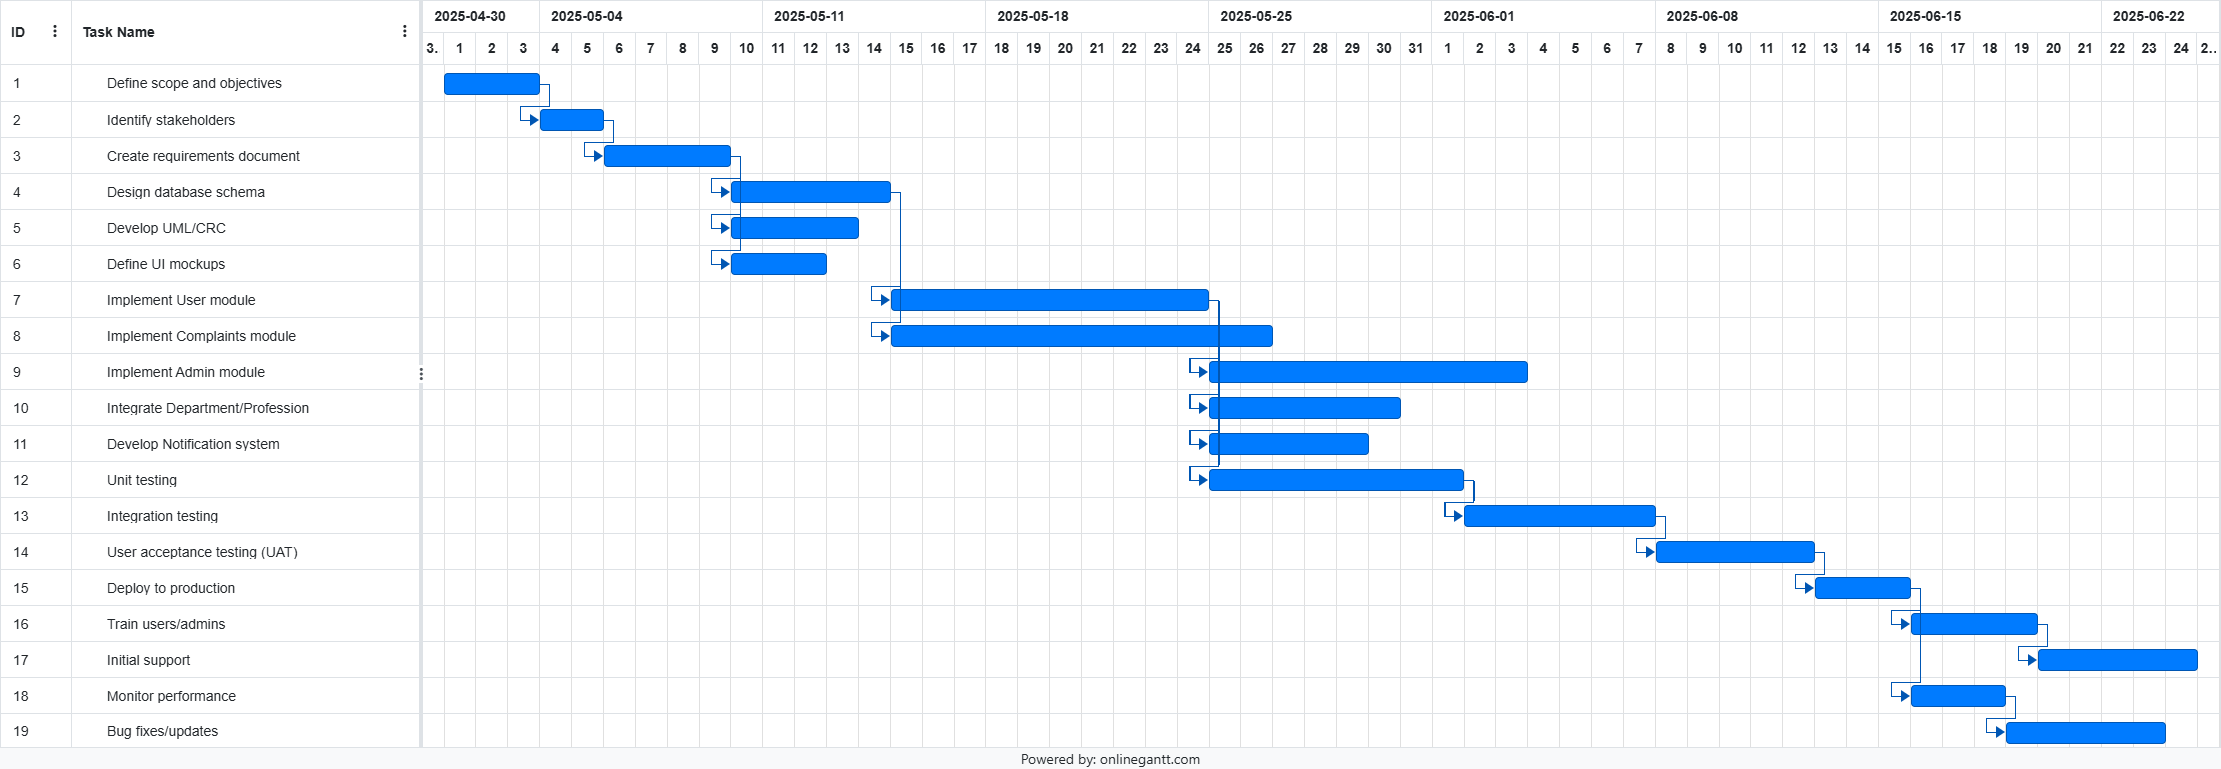
\includegraphics[width=1\linewidth]{photos/grant-chart.png}
    \caption{Grantt Chart}
    \label{fig:enter-label}
\end{figure}

\subsection{Project Estimation}
This section provides detailed estimates for the development of the Complaint Management System, tailored to a team of two members and a project of moderate complexity. The estimates include product size, effort, schedule, and cost, with justifications rooted in industry standards.
\\ \\ 
\textbf{Product Size} \\
The product size is estimated based on the system's scope, which includes 9 classes (e.g., User, Complaint, Department) with approximately 50 methods and 50 attributes, as derived from the class diagram and CRC model. Using the Lines of Code (LOC) metric, the system is projected to require 4000–5000 LOC, reflecting a moderate-sized application for a lab project. Alternatively, using Function Points (FP), an estimate of 30–40 FP is appropriate, considering the number of entities and basic functionalities such as complaint filing and user management. This range is justified by the system's limited scope, avoiding advanced features, and aligning with typical academic project sizes.

\textbf{Effort}\\
Effort is calculated using the COCOMO (Constructive Cost Model) basic model for organic projects, where Effort = a $\times$ (Size)$^b$, with $a = 2.4$ and $b = 1.05$. Assuming a size of 35 FP (midpoint of 30–40 FP), the effort is:
\[
\text{Effort} = 2.4 \times (35)^{1.05} \approx 87 \text{ person-hours}.
\]
For a team of two members, this translates to approximately 43.5 person-hours per member. Given a 20-hour workweek per member over the 57-day schedule, the total effort is adjusted to 5–6 person-months (assuming 160 hours per month), reflecting the project's moderate complexity and the team's small size. This adjustment accounts for learning curves and part-time commitment typical in a lab setting.

\textbf{Schedule}\\
The project schedule, determined by the Critical Path Method (CPM), is set at 57 days, starting from May 1, 2025, and ending on July 4, 2025. This duration encompasses all tasks, including requirement analysis, design, development, testing, and deployment, as outlined in the WBS and Gantt chart. The schedule is justified by the critical path's longest sequence (e.g., requirements to complaints module to testing), ensuring a realistic timeline for a two-member team with overlapping tasks like UML development and database design.

\textbf{Cost}\\
The cost is estimated based on the effort and an hourly rate suitable for a student project. Assuming a rate of \$15 per hour (reflecting a reasonable student or intern wage in 2025), and a total effort of 87 hours, the cost is:
\[
\text{Cost} = 87 \times 15 = \$1,305.
\]



\section{Risk Analysis}

This section identifies potential risks associated with the development of the Complaint Management System and outlines a Risk Mitigation, Monitoring, and Management (RMMM) plan to address them, tailored to a two-member team in an academic lab setting.

\subsection{Identify Risks (SWOT Analysis)}

A SWOT analysis evaluates the project's internal Strengths and Weaknesses, as well as external Opportunities and Threats.

\begin{itemize}
    \item \textbf{Strengths}: The team consists of two motivated students with basic software engineering knowledge, enabling efficient collaboration. The project's scope is well-defined through class modeling and project planning, providing a clear roadmap.
    \item \textbf{Weaknesses}: Limited team size (two members) may lead to workload imbalances or delays if one member is unavailable. Inexperience with complex integrations (e.g., notifications) could result in technical errors.
    \item \textbf{Opportunities}: The project offers a chance to gain practical experience with UML, DFDs, and project management tools, potentially enhancing skills for future courses or internships. Feedback from the instructor can improve the system design.
    \item \textbf{Threats}: Tight deadlines may pressure the team, risking incomplete testing. Unforeseen technical issues or resource constraints (e.g., limited access to tools) could hinder progress.
\end{itemize}

These factors highlight the need for proactive risk management to ensure successful project completion.

\subsection{ RMMM Plan}

The RMMM plan addresses identified risks with specific strategies for mitigation, monitoring, and management.

\begin{itemize}
    \item \textbf{Risk 1: Workload Imbalance Due to Small Team Size}
    \begin{itemize}
        \item \textbf{Mitigation}: Divide tasks evenly based on the WBS (e.g., one member handles design, the other development), with weekly progress reviews to reallocate if needed.
        \item \textbf{Monitoring}: Track task completion using a shared schedule (e.g., Gantt chart), checking progress every 3 days.
        \item \textbf{Management}: If one member falls behind, adjust deadlines or seek assistance from the instructor by May 17, 2025.
    \end{itemize}
    
    \item \textbf{Risk 2: Technical Errors in Integrations (e.g., Notifications)}
    \begin{itemize}
        \item \textbf{Mitigation}: Conduct unit testing for each module (e.g., User, Notification) early, using mock data to simulate interactions.
        \item \textbf{Monitoring}: Review integration test results by June 12, 2025, to identify issues.
        \item \textbf{Management}: Allocate extra time (e.g., 2 days) during the testing phase (June 4–11, 2025) to debug and consult online resources or peers if errors persist.
    \end{itemize}
    
    \item \textbf{Risk 3: Tight Deadline Pressure}
    \begin{itemize}
        \item \textbf{Mitigation}: Prioritize critical path tasks (e.g., Complaints module) and complete non-critical tasks (e.g., UI mockups) in parallel.
        \item \textbf{Monitoring}: Assess progress against the 57-day schedule weekly, with a final check by May 17, 2025.
        \item \textbf{Management}: If delays occur, focus on core functionalities (e.g., complaint filing) and document limitations for submission.
    \end{itemize}
    
    \item \textbf{Risk 4: Unforeseen Technical Issues or Resource Constraints}
    \begin{itemize}
        \item \textbf{Mitigation}: Set up a basic development environment (e.g., LaTeX, Inkscape) and test database connectivity by May 10, 2025.
        \item \textbf{Monitoring}: Check tool availability and system performance during the design phase (May 10–14, 2025).
        \item \textbf{Management}: Request institutional support (e.g., software licenses) or extend testing time (e.g., June 12–17, 2025) if issues arise.
    \end{itemize}
\end{itemize}

This RMMM plan ensures risks are addressed systematically, aligning with the project's timeline and team capacity.



\end{document}